\subsection{Captura de Movimientos}

\subsubsection{Introducción}
La captura de movimientos se realiza por medio de la obtención de puntos del cuerpo mediante el sensor Kinect, cuyas coordenadas son tridimensionales. Una vez que se obtienen los puntos, con ellos se analizan los ángulos de las extremidades del cuerpo en los planos XY y ZY. Asimismo se realiza un seguimiento de los puntos en el tiempo de realización del movimiento.\\

\subsubsection{Método de captura}
\label{sec:Captura}
El sensor Kinect nos proporciona un seguimiento de 20 puntos del cuerpo humano (articulaciones) tal como se muestra en la figura \ref{fig:SkeletonJoints} \nameref{fig:SkeletonJoints}, de los 20 puntos disponibles se eligieron los puntos que se muestran a continuación ya que se involucran en cada movimiento de técnica de Karate Do y al realizar un análisis de los ángulos entre ellos, se observa un cambio visible con respecto al tiempo.

\begin{itemize} \itemsep1pt \parskip0pt \parsep0pt
	\item Brazos
	\begin{itemize} \itemsep1pt \parskip0pt \parsep0pt
		\item Shoulder right
		\item Elbow right
		\item Wrist right
		\item Shoulder left
		\item Elbow left
		\item Wrist left
	\end{itemize}
	\item Piernas
	\begin{itemize} \itemsep1pt \parskip0pt \parsep0pt
		\item Hip right
		\item Knee right
		\item Ankle right
		\item Hip left
		\item Knee left
		\item Ankle left
	\end{itemize}
	\item Cuerpo
	\begin{itemize} \itemsep1pt \parskip0pt \parsep0pt
		\item Shoulder center
		\item Hip center
	\end{itemize}
\end{itemize}

\begin{figure}[h]%La h significa que la colocara cerca del texto
	\begin{center}
		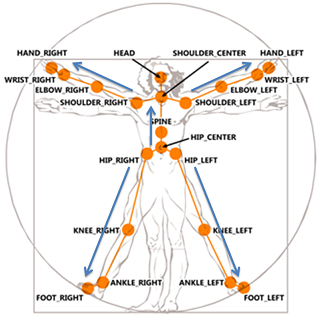
\includegraphics[scale=1]{./Figuras/Implementacion/SkeletonJoints}
	\end{center}
	\caption{Puntos del esqueleto de un humano}
	\label{fig:SkeletonJoints}
\end{figure}

La figura \ref{fig:AngulosXY} \nameref{fig:AngulosXY} muestra los ángulos analizados \textalpha, \textbeta, y \textgamma  que corresponden al seguimiento del movimiento de ambos brazos y de las piernas en el plano XY respectivamente. Estos ángulos cambian proporcionalmente al movimiento realizado.\\

Las figuras \ref{fig:AngulosYZ} \nameref{fig:AngulosYZ} muestran los ángulos analizados \textzeta, \texteta, y \texttheta  que corresponden al seguimiento del movimiento de ambos brazos y de las piernas en el plano ZY respectivamente. Estos ángulos cambian proporcionalmente al movimiento realizado.\\

El proceso de captura comienza analizando cada una de las posturas de inicio de los movimientos de técnica y se termina analizando cada una de las posturas finales. Esto nos permite capturar los ángulos en una serie de tiempo que varía con respecto al inicio y fin de la captura.\\

La información capturada se guarda en un archivo XML que contiene cada una de las series de ángulos en tiempo por cada extremidad y por cada plano. El archivo se guarda en el catálogo de la base de datos de movimientos de técnica.\\

\begin{figure}[H]%La h significa que la colocara cerca del texto
	\begin{center}
		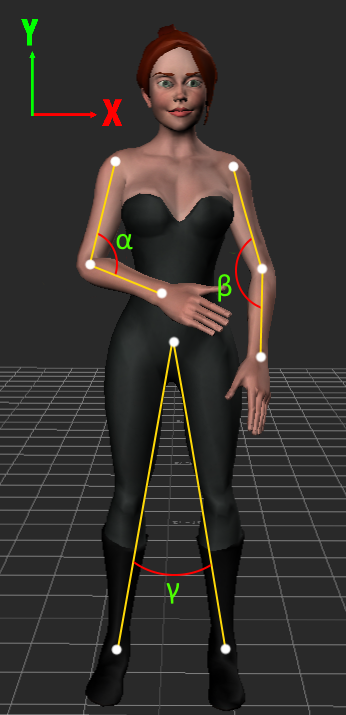
\includegraphics[scale=0.45]{./Figuras/Implementacion/AngulosXY}
	\end{center}
	\caption{Ángulos en el plano XY}
	\label{fig:AngulosXY}
\end{figure}

\begin{figure}[H]
	\centering
	\subfloat[Vista lateral derecha]{
		\label{fig:AngulosYZ1}
		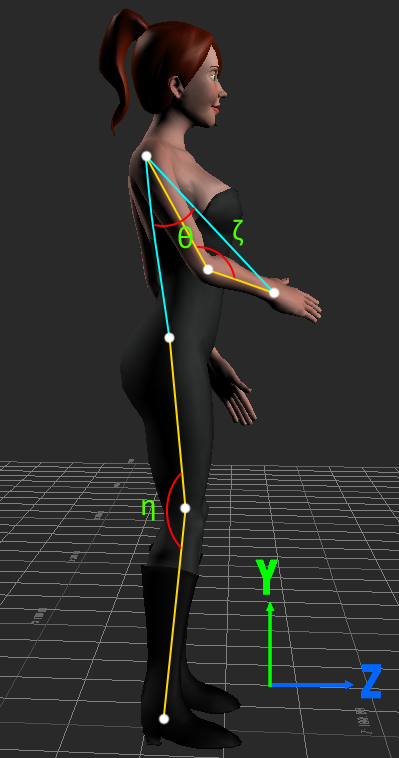
\includegraphics[scale=0.45]{./Figuras/Implementacion/AngulosYZ1}}
	\subfloat[Vista lateral izquierda]{
		\label{fig:AngulosYZ2}
		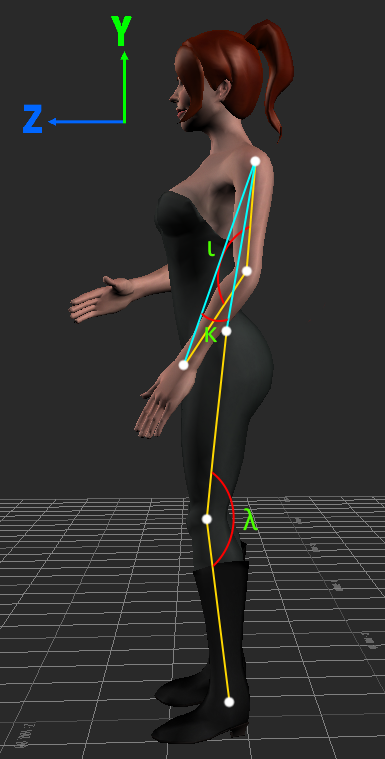
\includegraphics[scale=0.45]{./Figuras/Implementacion/AngulosYZ2}}
	\caption{Ángulos en el plano YZ}
	\label{fig:AngulosYZ}
\end{figure}

\subsubsection{Determinación del umbral}
\label{sec:Umbral}
Para conocer el valor del umbral, un Entrenador experto realizó todos los movimientos de técnica del catálogo, dichos datos fueron guardados en diferentes archivos para su posterior análisis.\\
Y asimismo replicó cada movimiento 9 veces. Para así poder compararlos por medio del algoritmo de Dynamic Time Warping con los primeros resultados que el mismo Entrenador guardó previamente. Y así poder conocer los resultados de la comparación de una misma persona, realizando los movimientos correctamente.\\

Estos fueron los resultados obtenidos:\\

Para calcular el umbral se usó la desviación estándar el cual es un índice numérico de la dispersión de un conjunto de datos. Mientras mayor es la desviación estándar, mayor es la dispersión de la población.\\
Se obtiene midiendo la diferencia entre cada valor del conjunto de datos y la media del conjunto de datos. Luego, sumando todas estas diferencias individuales para dar el total de todas las diferencias. Por último, dividiendo el resultado por el número total de observaciones para llegar a un promedio de las distancias entre cada observación individual y la media.\\

Este promedio de las distancias es la desviación estándar y de esta manera representa dispersión.\\

La fórmula de la desviación estándar es \begin{equation} s = \sqrt{\frac{1}{n} \sum_{i=1}^n \left(x_i - \bar{x}\right)^2} \end{equation}  donde \begin{equation} \sum_{i=1}^n \left(x_i - \bar{x}\right)^2 \end{equation} representa la suma de las diferencias al cuadrado entre cada observación y la media y N representa el número total de observaciones. \\

Al restar la media a los valores de cada observación individual para calcular las diferencias, los valores de las observaciones que están bajo la media producirán diferencias negativas, mientras que los valores de las observaciones que son mayores que la media proporcionarán valores positivos. Así, las diferencias positivas y negativas se compensarán entre sí y, en el caso de una distribución simétrica, producirán una suma igual a cero para la suma de las desviaciones individuales. Para evitar este problema, las desviaciones se elevan al cuadrado, de modo que todas las desviaciones sean positivas y se puedan sumar. Después, se calcula la raíz cuadrada para ‘compensar’, por decirlo así, la elevación al cuadrado anterior de los valores.\\

Una vez obtenidos los valores de la desviación estándar de cada extremidad, el valor del umbral se obtiene sumando dicha desviación estándar con la media respectiva de cada extremidad por cada movimiento.

%-------------------------------------------
A continuación se muestran los resultados obtenidos en los Movimientos: Senkuntsu - dachi Derecha y Senkuntsu - dachi Izquierda.\\

\textbf{Senkuntsu - dachi Derecha:}
La siguiente tabla muestra los valores que se generaron al comparar las 10 diferentes series de tiempo del Entrenador, en sus respectivos ángulos necesarios para la validación del movimiento de Senkuntsu - dachi Derecha, utilizando el algoritmo DTW.
\begin{figure}[H]%La h significa que la colocara cerca del texto
	\begin{center}
		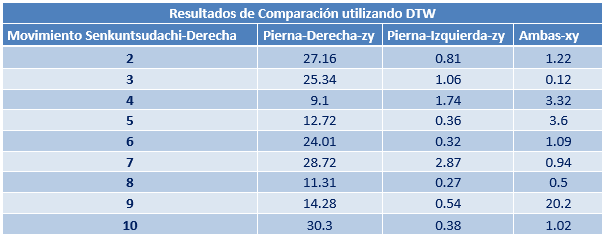
\includegraphics[scale=1]{./Figuras/Implementacion/Senkuntsudachi_Derecha_TablaDTW}
	\end{center}
	\caption{Tabla de resultados de la comparación de Senkuntsu - dachi Derecha}
	\label{fig:Senkuntsudachi_Derecha_TablaDTW}
\end{figure}
La siguiente tabla muestra los valores del promedio de los datos de la tabla anterior, así como la desviación estándar y los resultados del umbral (media más la desviación estándar).
\begin{figure}[H]%La h significa que la colocara cerca del texto
	\begin{center}
		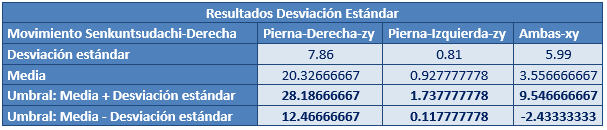
\includegraphics[scale=1]{./Figuras/Implementacion/Senkuntsudachi_Derecha_TablaDesvEstandar}
	\end{center}
	\caption{Tabla de los resultados del Umbral de Senkuntsu - dachi Derecha}
	\label{fig:Senkuntsudachi_Derecha_TablaDesvEstandar}
\end{figure}
Las siguientes gráficas muestran la desviación estándar y reflejan el valor del umbral.
\begin{figure}[H]
	\centering
	\subfloat[Desviación Estándar de Pierna Derecha]{
		\label{fig:Senkuntsudachi_Derecha_DesvEst_PiernaDer_zy}
		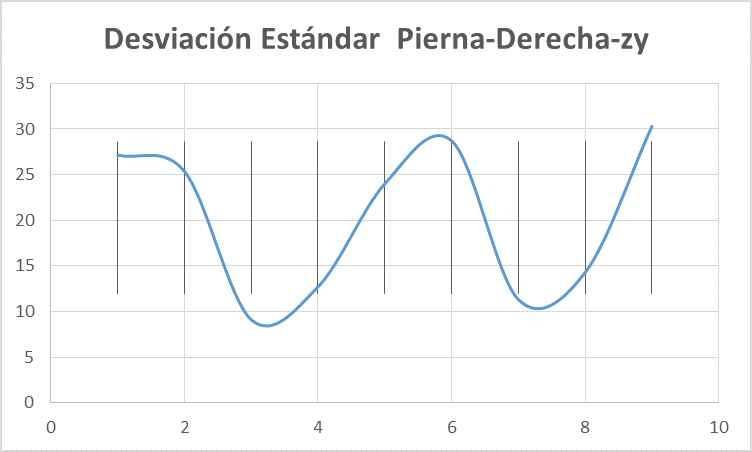
\includegraphics[scale=0.65]{./Figuras/Implementacion/Senkuntsudachi_Derecha_DesvEst_PiernaDer_zy}}
	\subfloat[Desviación Estándar de Pierna Izquierda]{
		\label{fig:Senkuntsudachi_Derecha_DesvEst_PiernaIzq_zy}
		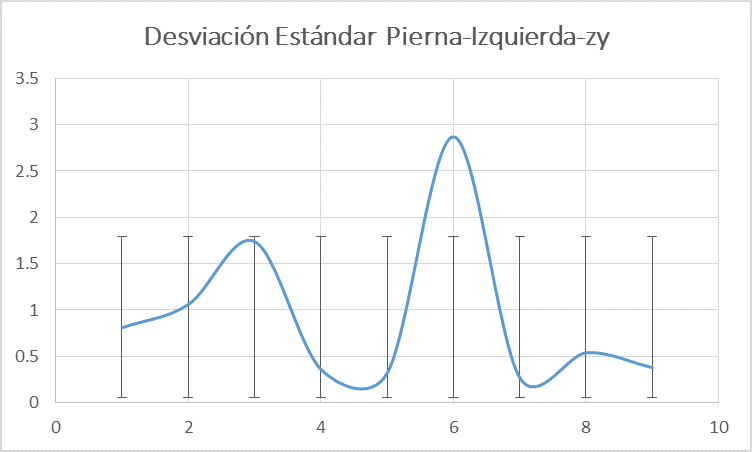
\includegraphics[scale=0.65]{./Figuras/Implementacion/Senkuntsudachi_Derecha_DesvEst_PiernaIzq_zy}}
	\caption{Desviación Estándar de Senkuntsu - dachi Derecha en ángulos en el plano YZ}
	\label{fig:DesvEstandar_Senkuntsudachi-Derecha}
\end{figure}
\begin{figure}[H]%La h significa que la colocara cerca del texto
	\begin{center}
		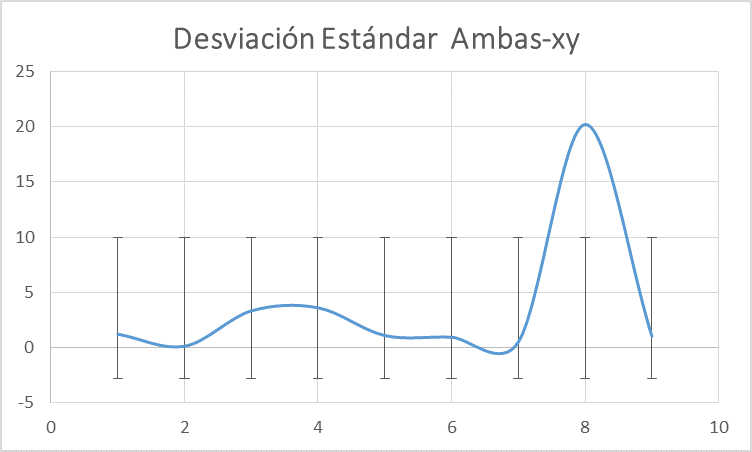
\includegraphics[scale=0.70]{./Figuras/Implementacion/Senkuntsudachi_Derecha_DesvEst_Ambas_xy}
	\end{center}
	\caption{Desviación Estándar del ángulo entre las dos piernas en el plano XZ}
	\label{fig:Senkuntsudachi_Derecha_DesvEst_Ambas_xy}
\end{figure}
%-------------------------------------------
\textbf{Senkuntsu - dachi Izquierda:}
La siguiente tabla muestra los valores que se generaron al comparar las 10 diferentes series de tiempo del Entrenador, en sus respectivos ángulos necesarios para la validación del movimiento de Senkuntsudachi Izquierda, utilizando el algoritmo DTW.
\begin{figure}[H]%La h significa que la colocara cerca del texto
	\begin{center}
		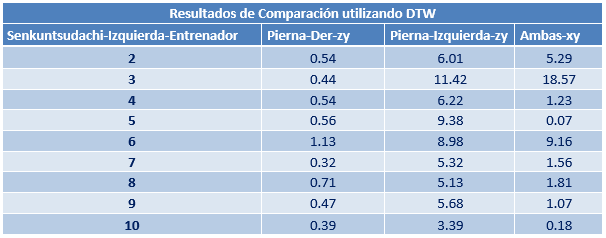
\includegraphics[scale=1]{./Figuras/Implementacion/Senkuntsudachi_Izquierda_TablaDTW}
	\end{center}
	\caption{Tabla de resultados de la comparación de Senkuntsu - dachi Izquierda}
	\label{fig:Senkuntsudachi_Izquierda_TablaDTW}
\end{figure}
La siguiente tabla muestra los valores del promedio de los datos de la tabla anterior, así como la desviación estándar y los resultados del umbral.
\begin{figure}[H]%La h significa que la colocara cerca del texto
	\begin{center}
		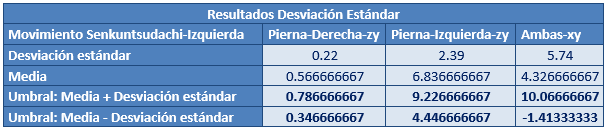
\includegraphics[scale=1]{./Figuras/Implementacion/Senkuntsudachi_Izquierda_TablaDesvEstandar}
	\end{center}
	\caption{Tabla de los resultados del Umbral de Senkuntsu - dachi Izquierda}
	\label{fig:Senkuntsudachi_Izquierda_TablaDesvEstandar}
\end{figure}
Las siguientes gráficas muestran la desviación estándar y reflejan el valor del umbral.
\begin{figure}[H]
	\centering
	\subfloat[Desviación Estándar de Pierna Derecha]{
		\label{fig:Senkuntsudachi_Izquierda_DesvEst_PiernaDer_zy}
		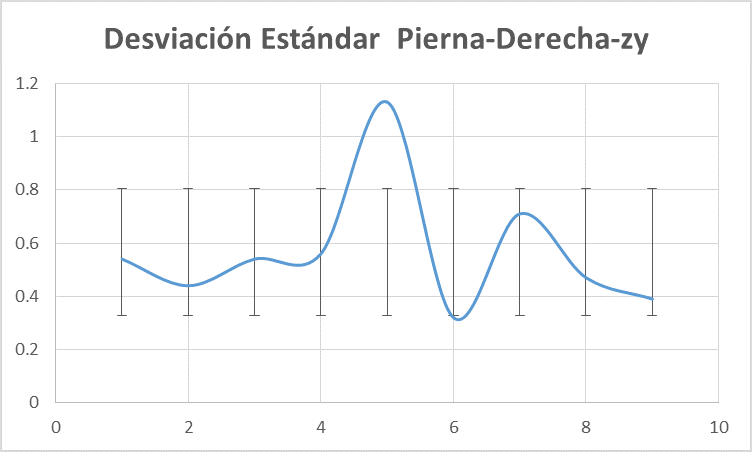
\includegraphics[scale=0.65]{./Figuras/Implementacion/Senkuntsudachi_Izquierda_DesvEst_PiernaDer_zy}}
	\subfloat[Desviación Estándar de Pierna Izquierda]{
		\label{fig:Senkuntsudachi_Izquierda_DesvEst_PiernaIzq_zy}
		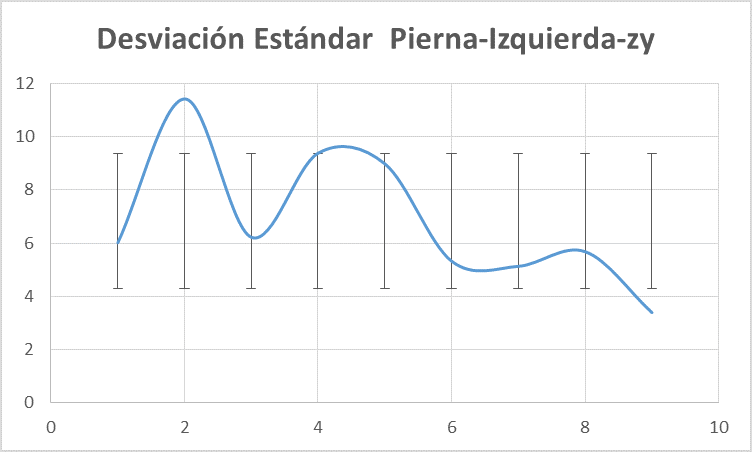
\includegraphics[scale=0.65]{./Figuras/Implementacion/Senkuntsudachi_Izquierda_DesvEst_PiernaIzq_zy}}
	\caption{Desviación Estándar de Senkuntsu - dachi Izquierda en ángulos en el plano YZ}
	\label{fig:DesvEstandar_Senkuntsudachi-Izquierda}
\end{figure}
\begin{figure}[H]%La h significa que la colocara cerca del texto
	\begin{center}
		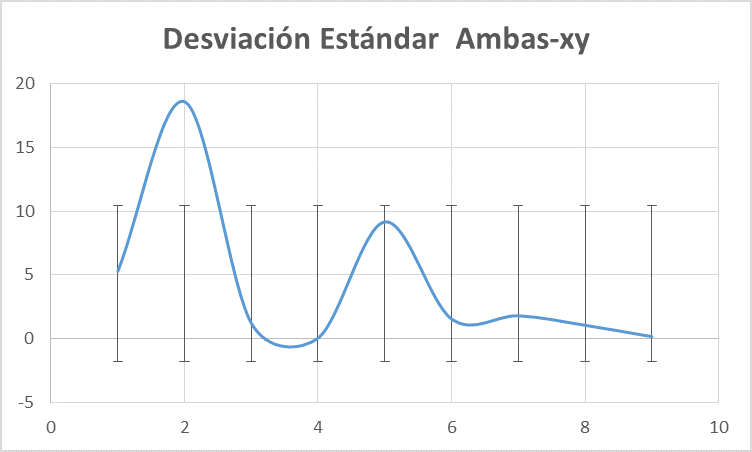
\includegraphics[scale=0.70]{./Figuras/Implementacion/Senkuntsudachi_Izquierda_DesvEst_Ambas_xy}
	\end{center}
	\caption{Desviación Estándar del ángulo entre las dos piernas en el plano XZ}
	\label{fig:Senkuntsudachi_Izquierda_DesvEst_Ambas_xy}
\end{figure}

%-------------------------------------------
\subsubsection{Errores y problemas de hardware}
Debido a las limitantes que presenta el sensor kinect,  cuando un punto llega a ``interponerse" frente a otro punto, hay ocasiones en donde los valores de los puntos involucrados se alteran, arrojando coordenadas erróneas, sin valor o con un valor no numérico. En consecuencia, al tomar un valor erróneo del punto al hacer el análisis del seguimiento de los diferentes ángulos con respecto a los puntos del cuerpo, el resultado del ángulo analizado se obtiene con un valor distinto al de la realidad.\\

Cuando ocurre algún error en la captura en la herramienta (como se mencionó previamente por un traslape, o incluso por la velocidad de movimiento), estos errores son visibles al mostrarse como un valor no numérico (o NaN por su nombre en inglés Not a Number) o como un campo vacío (no un valor Null); dichos errores, al poder ser analizados, si se llega a encontrar alguno de ellos, se muestra un mensaje en pantalla pidiendo al Entrenador repetir el movimiento para comenzar la captura nuevamente. Una vez que no se encontraron este tipo de errores de captura por hardware, se procede a guardar la información capturada para posteriormente ser utilizada en la validación de movimientos del Practicante.\\

Microsoft propone dentro de su documentación oficial del sensor Kinect el uso de los llamados ``smooth parameters", estos parámetros son parte de una función del SDK que permiten reducir los problemas en la interposición de puntos realizando un procesamiento mayor para calcular los puntos ``ocultos", este procesamiento como consecuencia tiene una mayor precisión pero reduce el tiempo de respuesta, es decir hay una latencia entre los movimientos que realiza el usuario y la respuesta en pantalla de la captura; en su contraparte sin el uso de los smooth parameters se reduce el tiempo de respuesta obteniendo un resultado de captura en tiempo real, pero perdiendo la precisión en la captura a la hora de las interposiciones de puntos. Para el caso de la herramienta realizada de acuerdo a las necesidades se optó por utilizar los smooth parameters para obtener una mejoría en los resultados.\\

Como ejemplo del uso de los smooth parameters en la herramienta, se realizó el análisis de la captura de un movimiento (Hachiji dachi), mostrando los resultados a continuación:\\

\begin{figure}[H]
	\begin{center}
		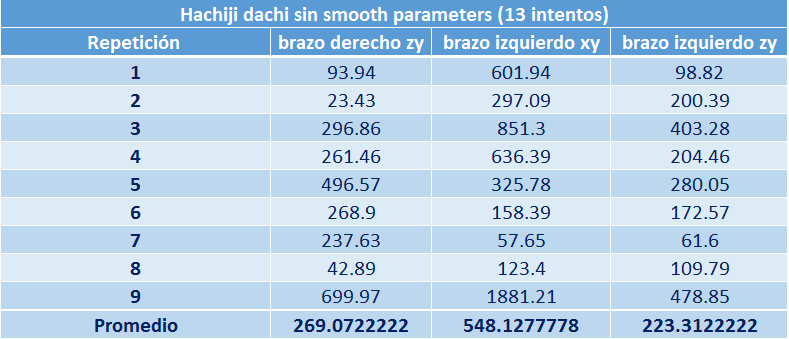
\includegraphics[scale=0.70]{./Figuras/Implementacion/SmoothParameters/HachijiDachiSinSmooth}
	\end{center}
	\caption{Captura del movimiento Hachiji-dachi sin el uso de los smooth parameters}
	\label{fig:Hachijidachi_sin_smooth_parameters}
\end{figure}
\begin{figure}[H]
	\begin{center}
		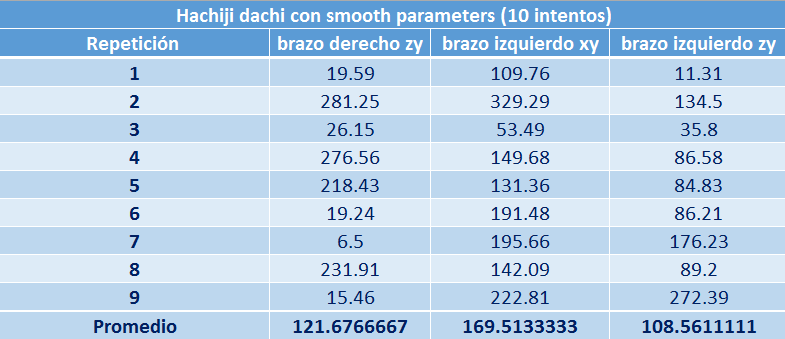
\includegraphics[scale=0.70]{./Figuras/Implementacion/SmoothParameters/HachijiDachiConSmooth}
	\end{center}
	\caption{Captura del movimiento Hachiji-dachi con el uso de los smooth parameters}
	\label{fig:Hachijidachi_con_smooth_parameters}
\end{figure}

Se obtuvo que los smooth parameters redujeron de forma considerable los valores de los umbrales del algoritmo DTW, además de que sin los parámetros se tuvieron que hacer 13 capturas para obtener 10 valores (ocurrieron 3 capturas erróneas que se tuvieron que recapturar), y por su contraparte con los parámetros las 10 capturas se realizaron de manera exitosa.\\


